\chapter{Background and Related Work}
\label{ch:background}

\section{Neural Network}
A neural network (also artificial neural network or neural net, abbreviated ANN
or NN) is a model inspired by the structure and function of biological neural networks
in animal and human brains.
\begin{figure}[H]
	\centering
	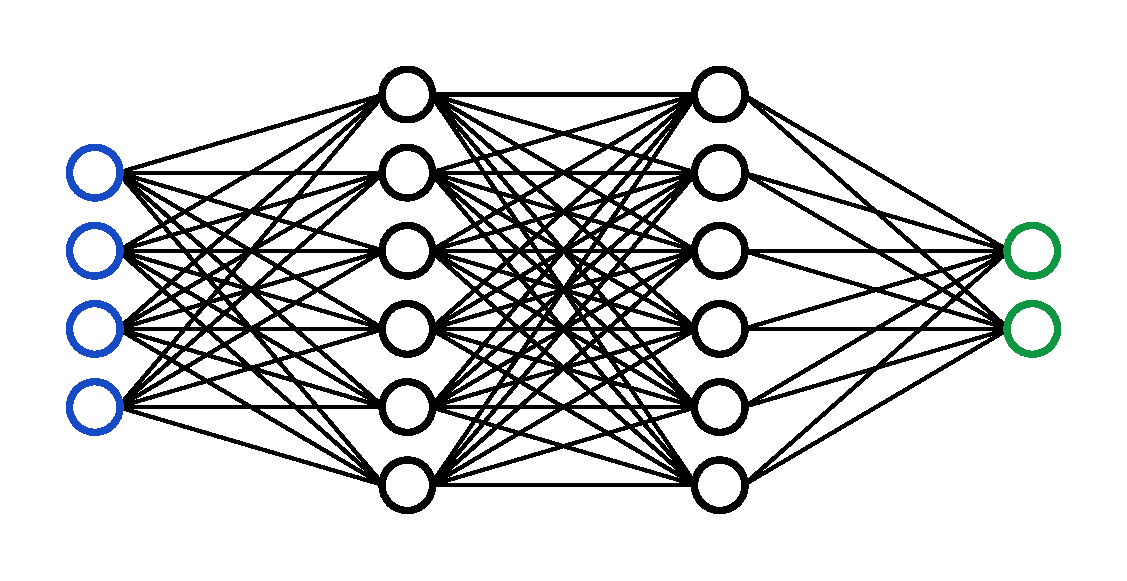
\includegraphics[width=1\linewidth]{images/network.eps}
	\caption{An example Neural Network. (from \cite{pic4nn})}
	\label{fig:nn}
\end{figure}
Neural networks consis of neurons organized into layers (see \autoref{fig:nn}), where the layers usually perform a linear transformation followed by a non-linear activation function. This allow networks to learn complex patterns and relationships in the data.
There are numerous different activation functions. We can put them into 2
category: Non-Linear Activate Functions and others.

\section{Non-Linear Activation Functions}
In this section, we will walk-through the most important activation functions, and their properties.

Sigmoid:
\begin{equation}
	f(x)=\frac{1}{1+e^{-x}}\label{sigmoid}
\end{equation}
It’s especially useful for classification or probability prediction tasks so
that it can be implemented into the training of computer vision and deep
learning networks. However, vanishing gradients can make these problematic when
used in hidden layers, and this can cause issues when training a model. That's why nowadays, ReLU (see \autoref{relu}) is more widely
used in computer vision and deep learning instead of Sigmoid.

\bigskip

Tanh:
\begin{equation}
	f(x)=\frac{\left(e^{x}-e^{-x}\right)}{\left(e^{x}+e^{-x}\right)}\label{tanh}
\end{equation}
It is a steeper gradient and also encounters the same vanishing gradient challenge
as sigmoid.

\bigskip

ReLU:
\begin{equation}
	f(x)=\max (0, x) \label{relu}
\end{equation}
ReLU does not activate every neuron in sequence at the same time, making it more
efficient than the tanh or sigmoid/logistic activation functions. Unfortunately,
the downside of this is that some weights and biases for neurons in the network
might not get updated or activated.

\bigskip

LeakyReLU:
\begin{equation}
	f(x)=\max (0.1*x, x) \label{leaky-relu}
\end{equation}
The advantages of Leaky ReLU are same as that of ReLU, in addition to the fact that
it does enable backpropagation, even for negative input values.

\bigskip

ParametricReLU:
\begin{equation}
	f(x)=\max (a*x, x) \label{para-relu}
\end{equation}
Parametric ReLU is another variant of ReLU that aims to solve the problem of
gradient’s becoming zero for the left half of the axis.

\bigskip

Softmax:
\begin{equation}
	\operatorname{softmax}\left(z_{i}\right)=\frac{\exp \left(z_{i}\right)}{\sum_{j}\exp
		\left(z_{j}\right)}\label{softmax}
\end{equation}
It is most commonly used as an activation function for the last layer of the
neural network in the case of multi-class classification.

\section{ARIMA}

Typical forecasting techniques in the literature utilize statistical tools, such
as exponential smoothing (ETS) \cite{gardner1985forecasting} and auto regressive
integrated moving average (ARIMA) \cite{SEMENOGLOU20211072}, on numerical time
series data for making one-step-ahead predictions. These predictions are then recursively
fed into the future inputs to obtain multi-step forecasts. Multi-horizon
forecasting methods \cite{taieb2010forecasting} and
\cite{marcellino2006comparison} directly generate simultaneous predictions for
multiple predefined future time steps.

\section{RNN - Recurrent Neural Network}

Recurrent neural networks (RNNs)
are designed to handle temporal
problems, and they are widely used
for sequential data and time-series
analysis. The RNN family is natural
choice for financial forecasting as
well, see e.g. \cite{Rumelhart1986}. Although RNN is able to accurately characterize the contextual relationship between sequential
data, this relationship weakens as the gap distance between them grows.

\autoref{fig:rnn} present the unfolded architecture of an RNN.

\begin{figure}[H]
	\centering
	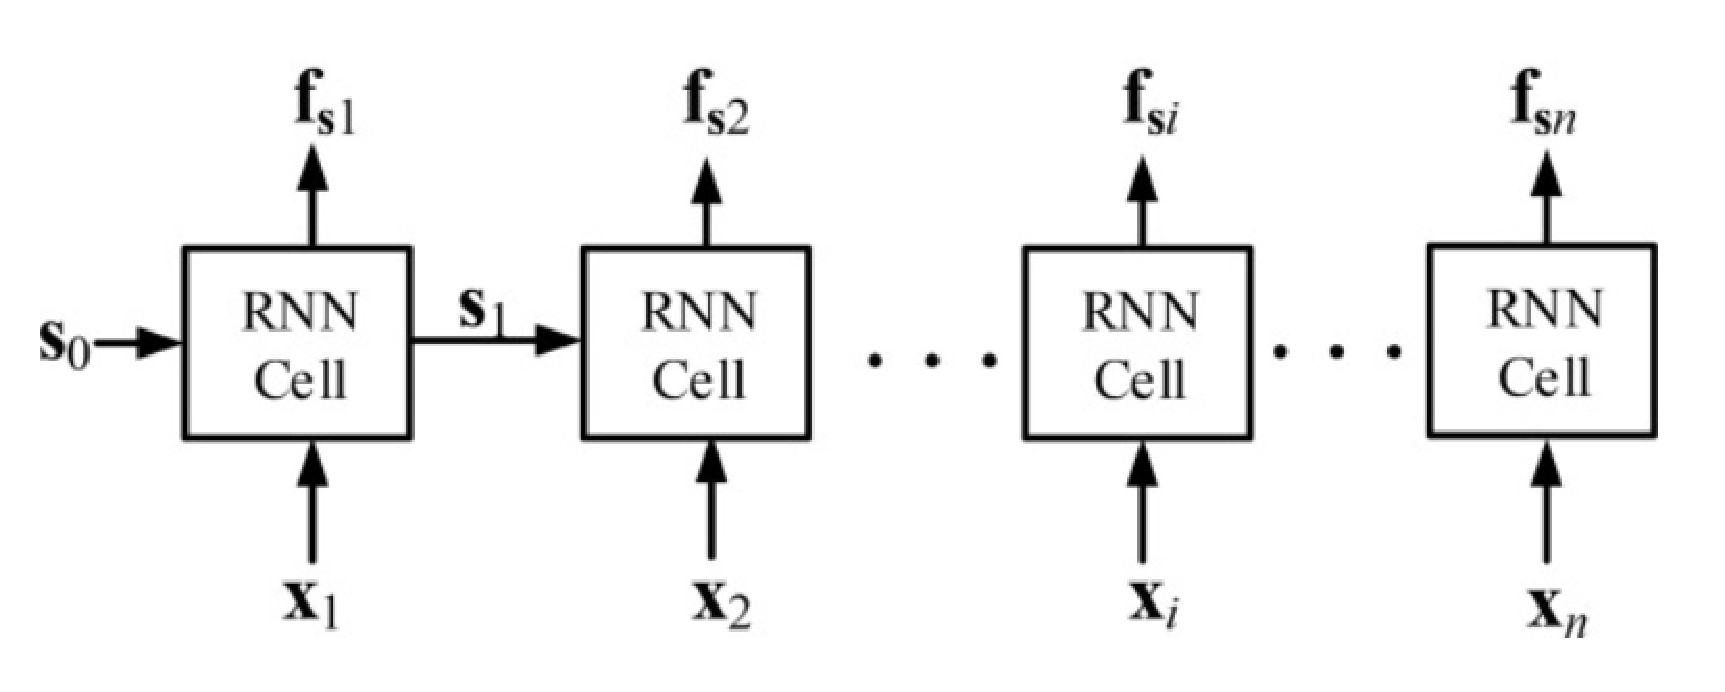
\includegraphics[width=1\linewidth]{images/rnn.eps}
	\caption{Recurrent Neural Network model. (from \cite{pic4rnn})}
	\label{fig:rnn}
\end{figure}

Moreover, an RNN model has the vanishing gradient problem for the long sequence
data. However, LSTM can prevent this problem during training.

\section{CNN - Convolutional neural network}

A convolutional
neural network (CNN) involves
special layers that perform
convolution and pooling. CNN
architectures serve as the most
widely used ANNs in image
processing and computer vision, but they are rarely used for financial.

\section{LSTM - Long Short-Term Memory}
Long Short-Term Memory (LSTM) is a special RNN that a memory mechanism with gates, making the network capable to learn long-term dependencies and preventing the vanishing gradient problem. The structure of an LSTM cell is demonstrated in \autoref{fig:lstm}.

\begin{figure}[H]
	\centering
	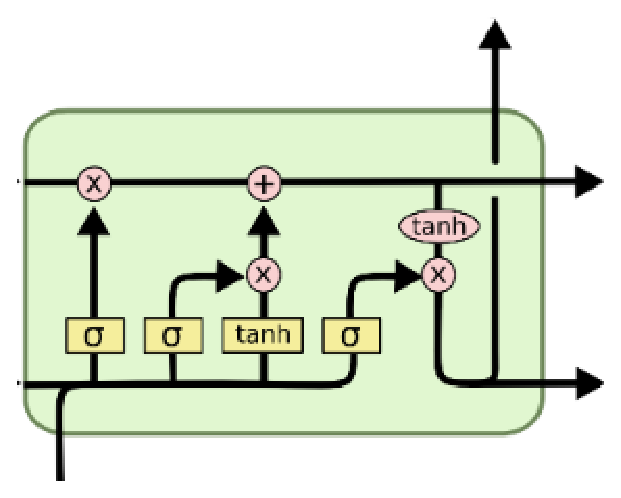
\includegraphics[width=0.6\linewidth]{images/lstm.eps}
	\caption{LSTM - Long Short-Term Memory architecture. (from \cite{pic4lstm})}
	\label{fig:lstm}
\end{figure}

LSTM \cite{6795963} is widely used for financial time series
prediction, particularly in forecasting stock prices. There are also many
variables of LSTM such as BiLSTM, Conv-LSTM \cite{Wang_2019} , Attentive – LSTM \cite{feng2019enhancing}
with an attention mechanism to predict stock price movement. However, \cite{DBLP:journals/corr/abs-1907-00235}
points out that LSTM can only distinguish 50 positions nearby with an effective context
size of about 200. That means that LSTM-based models suffer from the difficulty in
capturing extremely long- term dependencies in time series

\section{Time2Vec}

Time2Vec \cite{DBLP:journals/corr/abs-1907-05321} is an approach providing a
model – agnostic vector representation for time. Time decomposition technique that
encodes a temporal signal into a set of frequencies.

\begin{equation}
	t 2 v(\tau)[i]=\left\{
	\begin{array}{cc}
		w_i \tau+\varphi_i                    & \text{ if } i=0             \\
		\sin \left(w_i \tau+\varphi_i\right), & \text{ if } 1 \leq i \leq k
	\end{array}\right. \label{t2v}
\end{equation}
\smallskip

This design have three important properties:

\begin{enumerate}
	\item \label{step:first} Capturing both periodic and non periodic patterns.
	
	\item Being invariant to time re-scaling.
	
	\item Being simple enough so it can be combined with many models.
\end{enumerate}

The sin activation function is inspired parts of positional encoding from \cite{DBLP:journals/corr/VaswaniSPUJGKP17}
which can be combined with transformers model.

\section{Transformer}
The innovation of Transformer in deep learning \cite{DBLP:journals/corr/VaswaniSPUJGKP17}
has brought great interests recently due to its excellent performances in natural
language processing (NLP) \cite{devlin-etal-2019-bert}. Over the past few years,
numerous Transformers have been proposed to advance the state-of-the-art performances
of various tasks "significantly" Transformers have shown great modeling ability for
long- range dependencies and interactions in sequential data and thus are
appealing to time series modeling. Many variants of Transformer have been proposed
to address special challenges in time series modeling and have been successfully
applied to various time series tasks, such as forecasting anomaly detection and
classification \cite{wen2023transformers}.

\autoref{fig:transformer} shows the architecture of Transformer.

\begin{figure}[H]
	\centering
	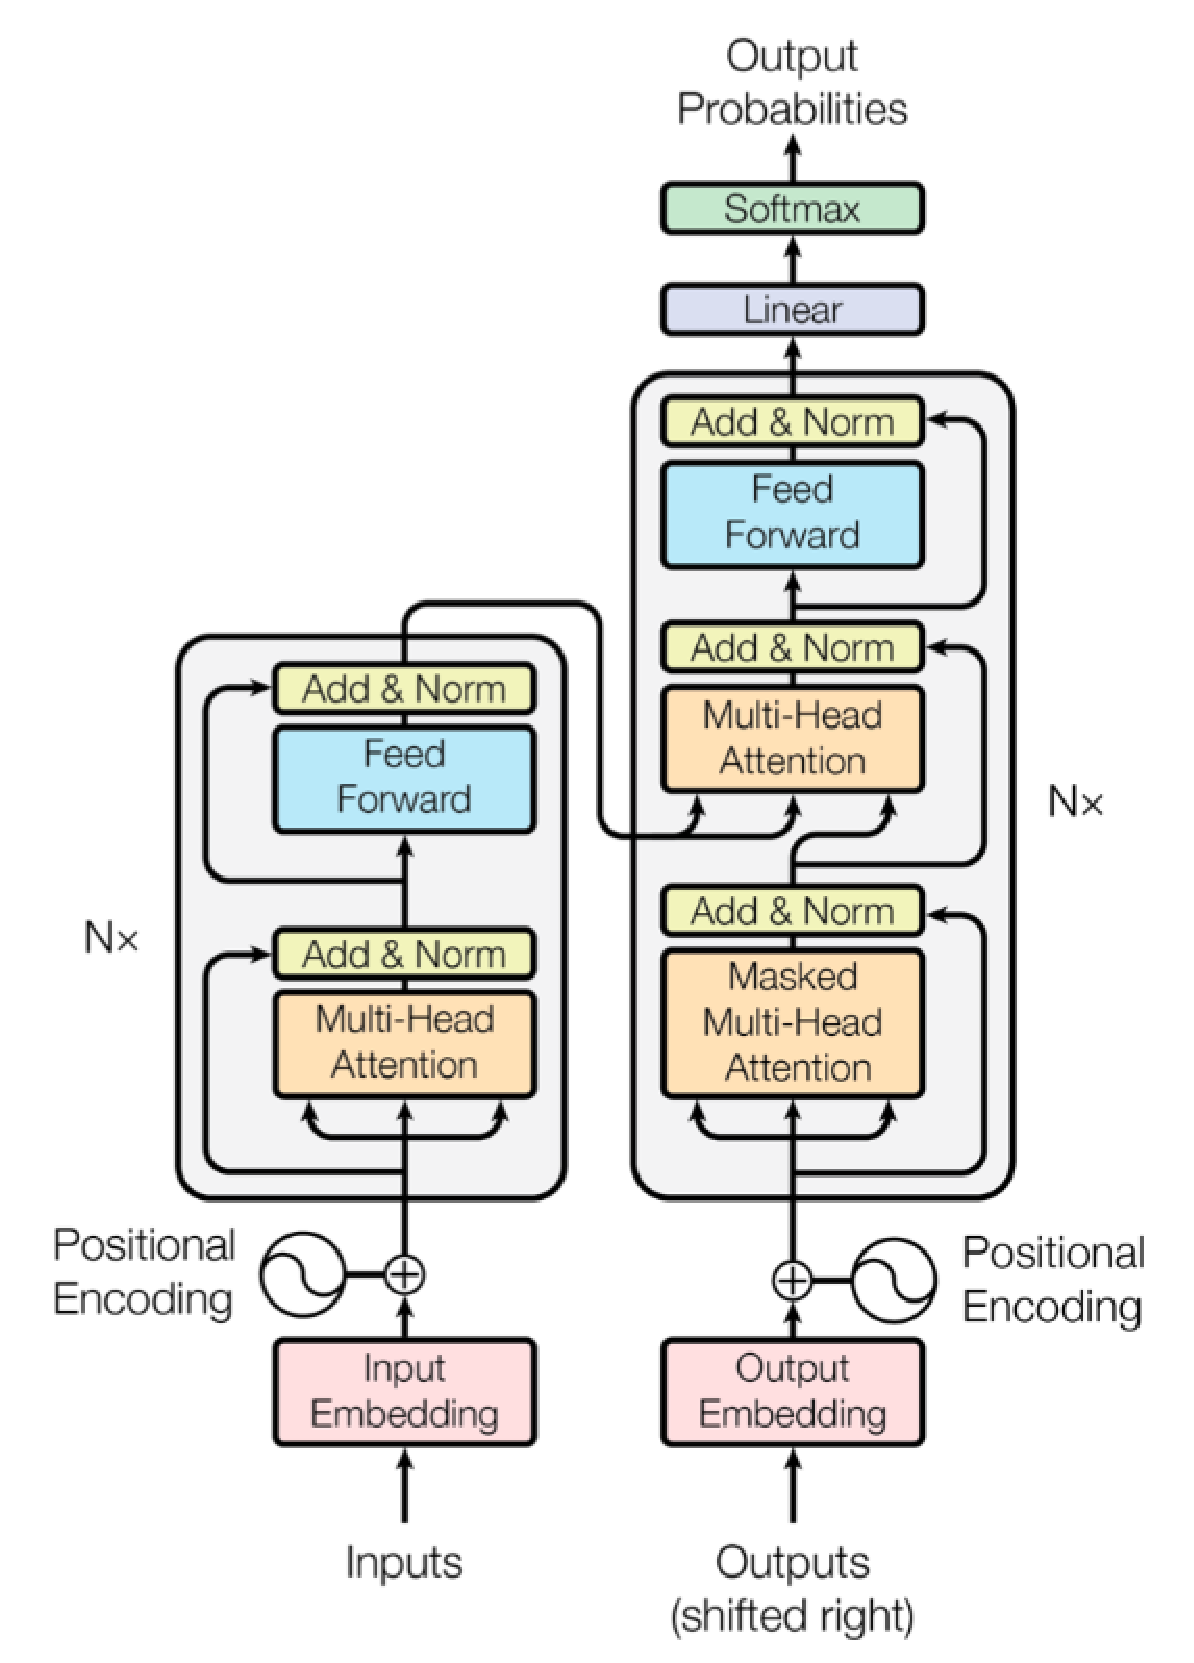
\includegraphics[width=0.65\linewidth]{images/trans.eps}
	\caption{The Transformer - model architecture. (from \cite{pic4trans})}
	\label{fig:transformer}
\end{figure}

\section{Transformer and Time-Embedding}

Unlike natural language data where positional encoding suffices to capture word
order, processing sequential data with Transformers necessitates a nuanced approach
to extract temporal dependencies. This gap is bridged by Time Embedding, which imbue
the model with an understanding of chronological order, preventing nonsensical
predictions where distant historical prices hold equal sway as recent ones. To address
the temporal challenges inherent in Transformers, the Time2Vec methodology is
adopted, offering a model-agnostic vector representation of time. This approach
encapsulates both periodic and non-periodic patterns while maintaining invariant
to time re-scaling, ensuring the model's ability to comprehend and utilize temporal
features effectively in predicting stock prices.

\section{Optimizer}
In supervised learning, the training of ANNs are usually carried out as a data-driven numerical optimization o
a lost function. In feedforward NNs, where the neurons are organized in layers, backpropagation and a stochastic gradient descent optimizer are mainly used. There are an enormous optimizer out there, but in this thesis, we are using Adam
Optimizer.

\subsection{Adaptive Moment Estimation}
Adaptive Moment Estimation is an algorithm for optimization technique for gradient
descent. The method is really efficient when working with large problem
involving a lot of data or parameters. It requires less memory and is efficient.
Intuitively, it is a combination of the ‘gradient descent with momentum’ algorithm
and the ‘RMSP’ algorithm. Adam Optimizer inherits the strengths or the positive
attributes of the two methods and builds upon them to give a more optimized
gradient descent.

\subsection{Momentum}
This algorithm is used to accelerate the gradient descent algorithm by taking
into consideration the ‘exponentially weighted average’ of the gradients. Using averages
makes the algorithm converge towards the minima in a faster pace.

\subsection{Root Mean Square Propagation - RMSP}
Root mean square prop or RMSprop \cite{rmsp} is an adaptive learning algorithm that tries to
improve AdaGrad \cite{ada}. Instead of taking the cumulative sum of squared gradients like
in AdaGrad, it takes the ‘exponential moving average’.

\section{Evaluation metrics}
In this section we overview the most important metrics that are used to evaluate the performance of the predictions of a forecasting method.

\subsection{MAPE - Mean Absolute Percentage Error}
\label{mape}
Also known as mean absolute percentage deviation (MAPD), is a measure of
prediction accuracy of a forecasting method in statistics. It usually expresses the
accuracy as a ratio defined by the formula.
\begin{equation}
	\text{ MAPE }=\frac{1}{n}\sum_{i=1}^{n}\left|\frac{Y_{i}-\hat{Y}_{i}}{Y_{i}}\right| 
\end{equation}

$Y_{i}$: Actual value.

$\hat{Y}_{i}$: Predicted value.

$n$: number of values.

\subsection{MAE - Mean Absolute Error}
\label{mae}
Mean absolute error (MAE) is a measure of errors between paired observations expressing
the same phenomenon.
\begin{equation}
	\text{ MAE }=\frac{1}{n}\sum_{i=1}^{n}\left|Y_{i}-\hat{Y}_{i}\right| 
\end{equation}

$Y_{i}$: Actual value.

$\hat{Y}_{i}$: Predicted value.

$n$: number of values.

\subsection{RMSE - Root Mean Square Error}
\label{rmse}
Root mean square error (RMSE) is the residuals' standard deviation, or the average
difference between the projected and actual values produced by a statistical model.
\begin{equation}
	\mathrm{RMSE}=\sqrt{\sum_{i=1}^{n}\frac{\left({Y}_i-\hat{Y}_i\right)^2}{n}}
\end{equation}

$Y_{i}$: Actual value.

$\hat{Y}_{i}$: Predicted value.

$n$: number of values.

\subsection{MSE - Mean Square Error}
\label{mse}
Mean squared error (MSE), the average squared difference between the value
observed in a statistical study and the values predicted from a model.
\begin{equation}
	\mathrm{MSE}=\frac{1}{n}\sum_{i=1}^{n}\left(Y_{i}-\hat{Y}_{i}\right)^{2}.
\end{equation}

$Y_{i}$: Actual value.

$\hat{Y}_{i}$: Predicted value.

$n$: number of values.

\subsection{R2 - R-Square}
\label{r2}
R-Squared value shows how well the model predicts the outcome of the dependent
variable. R-Squared values range from 0 to 1. Squared value of 0 means that the model
explains or predicts 0\% of the relationship between the dependent and
independent variables.
\begin{equation}
	R^{2}=1-\frac{\sum\left(Y_{i}-\hat{Y_i}\right)^{2}}{\sum\left(Y_{i}-\bar{Y}\right)^{2}}
	.
\end{equation}

$Y_{i}$: Actual value.

$\hat{Y}_{i}$: Predicted value.

$\bar{Y}$: Mean of all values.

$n$: number of values.